\input{configuration}

\title{Lecture 21 --- Power Management and Energy-Aware Scheduling}

\author{Jeff Zarnett \\ \small \texttt{jzarnett@uwaterloo.ca}}
\institute{Department of Electrical and Computer Engineering \\
  University of Waterloo}
\date{\today}


\begin{document}

\begin{frame}
  \titlepage
\end{frame}


\begin{frame}
\frametitle{Power Consumption}

\begin{center}
	
\includegraphics[width=0.5\textwidth]{images/thepower.jpg}
\end{center}

Motivating why we should care about power consumption is easy.

The consumer market for buying laptops that last only an hour is tiny.\\
\quad Would you get a phone that doesn't last the day?

\end{frame}


\begin{frame}
\frametitle{Resource Management}

Even if we're not talking about running on battery, electricity has some cost to it.

\begin{center}
	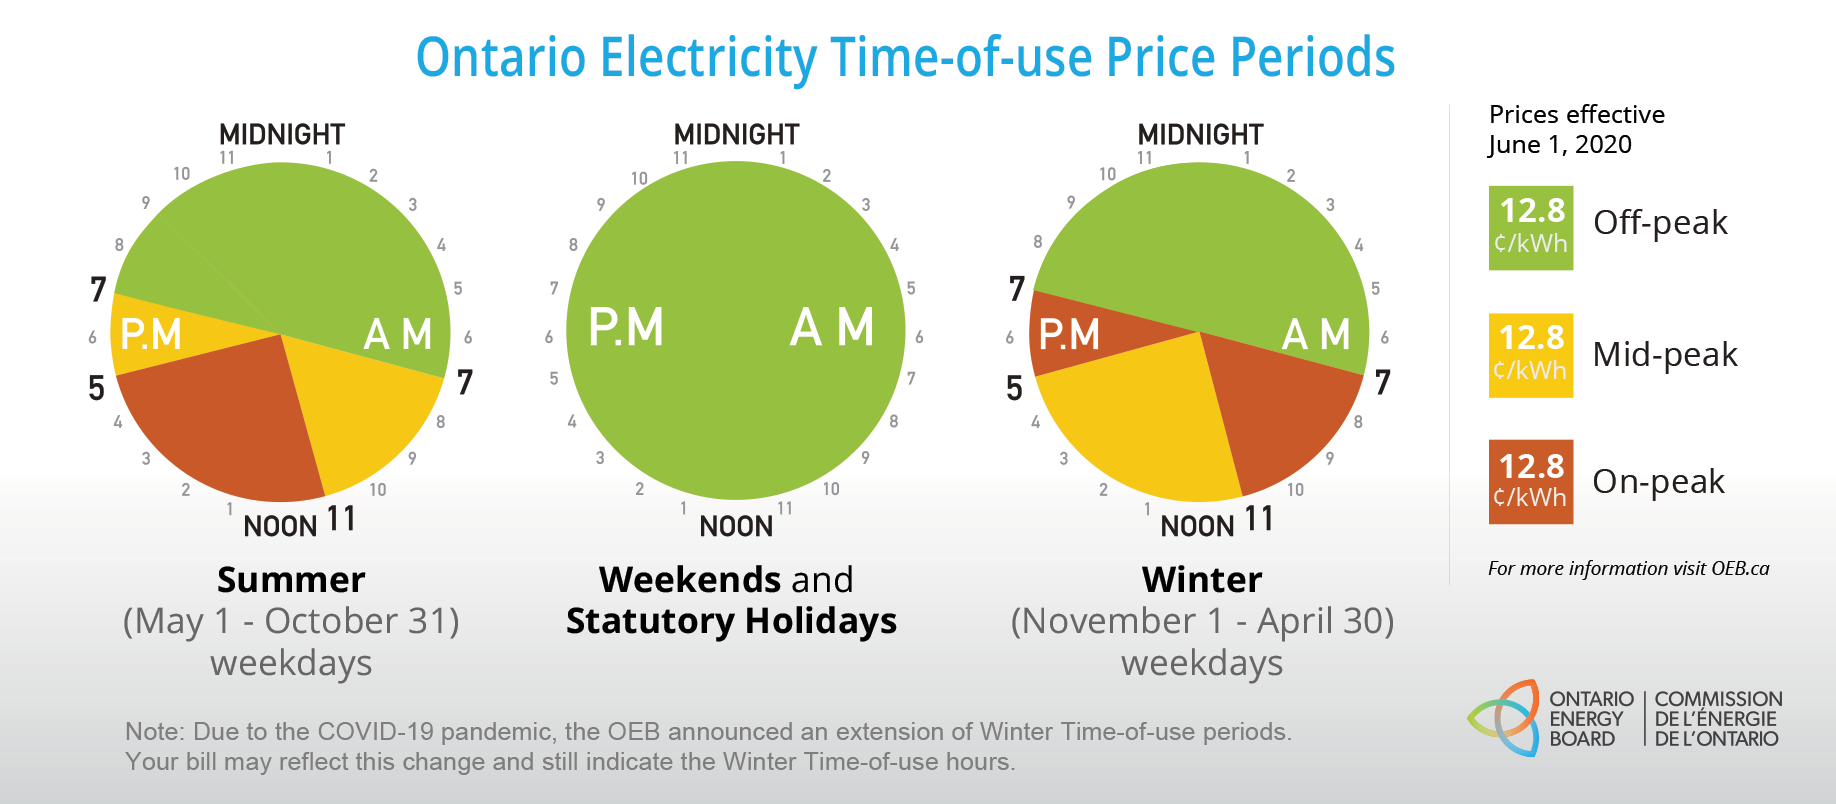
\includegraphics[width=0.7\textwidth]{images/tod.png}
\end{center}

Energy is a resource, and something the operating system can manage.

\end{frame}


\begin{frame}
\frametitle{ACPI and CPU}

Operating systems can discover and configure power states through a standard interface called \alert{ACPI}: Advanced Configuration and Power Interface.

We'll restrict the discussion to managing the power state of the CPU. 
\end{frame}


\begin{frame}
\frametitle{ACPI States}

It's also important to differentiate this discussion from the general ACPI states of the device (i.e., the laptop as a whole).

\begin{center}
	
\includegraphics[width=0.4\textwidth]{images/closedlid.jpg}
\end{center}

The ACPI states are the ones the user typically thinks of: powered off, powered on, sleeping, and hibernating (off but state stored to disk to restore on wake-up). 

\end{frame}


\begin{frame}
\frametitle{Full Power}

There are certainly times where we want to use the CPU to its maximum power. 

\begin{center}
	
\includegraphics[width=0.4\textwidth]{images/maximumwarp.jpg}
\end{center}

Play a game, render a video, execute a simulation, etc.

\end{frame}


\begin{frame}
\frametitle{Ahead Warp Factor Two}

You already know one reason why we should not run the CPU at 100\% at all times from the title of this topic: energy consumption and therefore battery life.


Heat can be uncomfortable if it's the laptop in your lap.

Heat is the enemy of reliability!

\end{frame}


\begin{frame}
\frametitle{Run, Forrest, Run}

For the CPU to be at 100\% is like running everywhere you go.\\
\quad Run to class, run to the lab, run to lunch... 
 
You \textit{can} do it, sure, but this depletes your energy way faster than walking and on a hot day you will definitely start feeling the negative effects of the heat. 

Instead, you adapt your pace of travel to the urgency of the situation and the state of resources.

\end{frame}

\begin{frame}
\frametitle{P-States and C-States}

The CPU has what are referred to as P-States and C-States.\\
\quad  P is for ``performance'' and C is for ``CPU idle''.

 P-States control the voltage and CPU frequency and C-States determine what the CPU does to reduce power consumption when no code is running (idle).

We're going to look at Intel Xeon. Other CPUs have similar behaviour.

\end{frame}


\begin{frame}
\frametitle{We Have Two Levers}

So, we have two levers available to reduce power consumption. 

\begin{center}
	
\includegraphics[width=0.5\textwidth]{images/volume-up.png}
\end{center}

Performance level and turning things off.

\end{frame}


\begin{frame}
\frametitle{P-States}

The first is the performance level setting, which says what clock speed we want to run the CPU at. 

This works because, to a first approximation: $P ~\propto~f V^{2}$ (oversimplifying a bit).

A small amount of hardware knowledge helps in explaining why.

\end{frame}

\begin{frame}
\frametitle{Twinkle, Twinkle Little Star}

Electromagnetism course: $P = V\times I$ so increasing the voltage very obviously would increase the power consumption.

The less-obvious component of this is that increasing the frequency is going to require a higher voltage to drive the components faster. 
 
 This is why CPU clock speeds today are about the same as they were in 2005.

\end{frame}


\begin{frame}
\frametitle{P-States}

P states are numbered: \texttt{P0} is maximum frequency.

Any other number is slower; higher numbers are slower CPUs.

 The more modern multi-core CPUs permit having different power states for different cores.

\end{frame}



\begin{frame}
\frametitle{Go Slower}

So, one way that we can immediately see improvement on power consumption is to set a higher-numbered P-state for the CPU and therefore run the CPU slower. 

Some do this automatically. Or it can be activated manually.

\begin{center}
	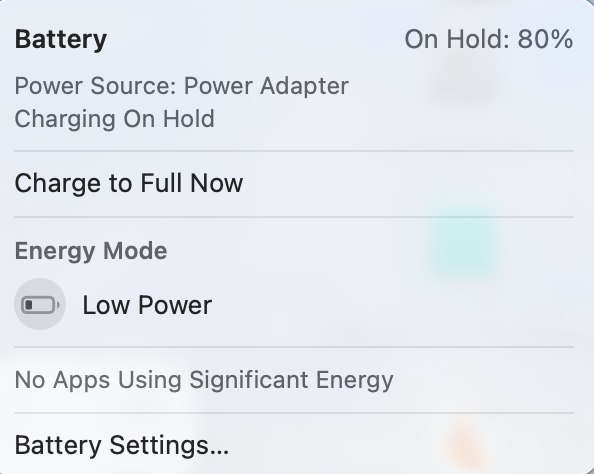
\includegraphics[width=0.4\textwidth]{images/lowpower.png}
\end{center}

\end{frame}


\begin{frame}
\frametitle{Oversimplifying}

Going to low power mode changes more than the clock speed of the CPU.

It also changes things like how often apps are permitted to refresh data in the background.

We'll come back to that later in this topic.

\end{frame}


\begin{frame}
\frametitle{Boost Mode}

Some CPUs also offer ``boost'' power where clock speed exceeds the nominal maximum for short periods of time. 

This only works when the chip is cool enough to do this without exceeding its heat limit, because the heat increases quite rapidly in this mode. 

This can, however, provide a meaningful performance boost that reduces latency if the workload is short but intense.

\end{frame}


\begin{frame}
\frametitle{C-States}

C-States are shutting down parts of the processor not currently being used.

\begin{center}
	
\includegraphics[width=0.7\textwidth]{images/leavetheroom.jpg}
\end{center}

\end{frame}

\begin{frame}
\frametitle{C-States}

C-States are numbered, with \texttt{C0} meaning everything is turned on and actively executing instructions. 

Any higher number than that means turning some things off.

The ACPI standard 6.4 names 4 states.

\end{frame}


\begin{frame}
\frametitle{C-States}

\begin{itemize}
	\item C0: CPU is executing instructions and running normally.
	\item C1: CPU is halted (not executing instructions) but maintains cache and can resume very quickly if needed.
	\item C2: Lower-power than C1 and takes more time and higher transition energy cost to wake back up to C0 than from C1.
	\item C3: Even lower-power than C2, caches not kept up to date, slowest time and highest energy cost to return to C0 state.
\end{itemize}


\end{frame}

\begin{frame}
\frametitle{Oversimplifying Again}

As with the P-states, modern multicore CPUs often have many more states than the minimum the spec requires.

It's hard to do a real demo of this because it requires loading a kernel module. 

We might be able to get an idea of it by looking at this CoreFreq GitHub project: \url{https://github.com/cyring/CoreFreq}.

\end{frame}


\begin{frame}
\frametitle{Race to Idle}

Discussion question: should we go fast temporarily and get to the idle state sooner, or go slower for a longer period of time? 

 What factors would we need to know to answer that?

\end{frame}


\begin{frame}
\frametitle{Race to Idle}

You can imagine this as $t_1 \times e_1$ (``race to idle'') vs $t_2 \times e_2$ (``slowdown'').

\begin{center}
	
\includegraphics[width=0.4\textwidth]{images/tortoise-hare.jpg}
\end{center}

It's tempting to say that lower and slower produces the best results (this might be true for cooking), but that's not always true. 

\end{frame}


\begin{frame}
\frametitle{Race to Idle}

Of course the correct answer is: it depends!

Customizing the approach can net something like 13-18\% energy savings. 

One of the most important determining factors is leakage.\\
\quad Intel CPUs have really high leakage!

\end{frame}


\begin{frame}
\frametitle{It's Bed Time}

If there is demand for the CPU, then the operating system may need to wake up a sleeping core (send it back to the C0 state). 

It can similarly send things to sleep with instructions. 

Hardware interrupts can also wake up a sleeping core. 

So when do we send cores to sleep? That's a really interesting topic.


\end{frame}


\begin{frame}
\frametitle{Energy-Aware Scheduling}

It's the scheduler making choices that reduce energy usage. 

We can break this down into a few different areas! 

Sending cores to sleep \& waking them up, choosing which cores are active at all, and managing background data \& refreshes.

\end{frame}


\begin{frame}
\frametitle{Go To Sleep}

The OS can issue commands to the cores to send them to sleep.

The idle task may contain the \texttt{HLT} (halt) instruction which puts it in C1.

\begin{center}
	
\includegraphics[width=0.5\textwidth]{images/gotosleep.jpg}
\end{center}

Send it only if we won't be using the core for a while.

\end{frame}


\begin{frame}
\frametitle{I'm Sleeping}

Putting a core to sleep (C1 or above) means the scheduler should not schedule threads to run on that core because it's not really ready to run threads right now. 

If demand increases, wake up cores again.

Interrupts send a core back into C0.

\end{frame}


\begin{frame}
\frametitle{But How}

Kernel docs: ``The role of the governor is to find an idle state most suitable for the conditions at hand.''

The description of each idle state, from the view of the governor, involves two figures: target residency and worst-case exit latency. 

Enter the idle state only if it's sensible.

\end{frame}


\begin{frame}
\frametitle{Scheduler Interrupt}

The scheduler interrupt is something that the kernel should handle differently than other timers. 

A different timer is for a specific event to be finished, but the scheduler one is specifically to run the scheduler. 

If there's nothing to do and CPUs are idle, then waking up the low-power CPU just for it to run the scheduler and decide to go back to sleep is a little wasteful.

\end{frame}


\begin{frame}
\frametitle{Governor Implementation}

We'll look at one example, called the \texttt{menu} governor.

It uses past data to predict the idle duration, and then uses the output of that calculation to select the best idle state.

Use the last 8 observed idle duration values; if the variance is small or small relative to the average, use that value, otherwise drop outliers and try again. 

Once an estimate is reached, then the governor can look at the list of idle states and choose the best match based on the target residency and exit latency.

\end{frame}


\begin{frame}
\frametitle{Big Cores and Little Cores}

A twist on SMP that is common in mobile devices: heterogeneous CPU topology.\\
\quad We have cores of different size and power.

\begin{center}
	
\includegraphics[width=0.4\textwidth]{images/biglittle.jpg}
\end{center}

They are still general purpose CPUs. They are just not identical.

\end{frame}


\begin{frame}
\frametitle{Where Do We Assign It}

The scheduler effectively has to guess where it should assign work to minimize the energy consumption without lowering performance (too much). 

It is easy enough for the kernel to have a good idea of what the capacity (performance capabilities) is for each kind of core. 

Similarly, the kernel has plenty of information about how much work there is to do right now and how busy each core is. 

The unknown variable is, how big is the thing to do?


\end{frame}


\begin{frame}
\frametitle{Big and Little Cores}

If the task is estimated to be ``too big'', it will have to go to a big core.

Smaller tasks could go to either one.

It is probably also task-nature-dependent.

Kernel implementers seem to agree: they look at past history with normalization.

\end{frame}


\begin{frame}
\frametitle{Can Go Either Place}

Let's imagine the specific task being considered now is small enough that it could go in a little or big core. 

The scheduler will find the CPU with the lowest usage in each of the size classes. 

For each of those, guess what the energy consumption would be, and select the one with the lowest predicted cost. 

\end{frame}

\begin{frame}
\frametitle{No Time To Lose}

There's a threshold where the kernel stops trying to do the energy-aware scheduling: 80\% utilization. 

Once demand is that high, trying to save energy is out the window since it probably won't help much and wastes time. 


\end{frame}



\begin{frame}
\frametitle{Hold On Now}

 In the settings of your phone you can choose whether apps are permitted to refresh in the background or if they can use cellular data (or only wifi). 
 
 You could do this intentionally to save battery -- but you probably don't want to limit it for everything. 

 
 Turning it off for social media seems sensible -- when you open the app it will show you whatever ads it was going to show you anyway.
 
 But you don't want to miss important notifications from messaging apps. 

\end{frame}


\begin{frame}
\frametitle{Middle Setting}

There is also sometimes a middle setting that defers work until later! 

iOS, for example, introduced the ability for background tasks to be deferred until later, such as when the device is plugged into the charger.

The nature of the task determines what conditions need to be true to execute the deferred task: presence of WiFi, being on the charger, time of day, et cetera. 

\end{frame}


\begin{frame}
\frametitle{Android Guide}

The Android developer guide does suggest batching or bundling operations. 

If the radio of your mobile device is off, it takes some time and energy to turn it on and connect. 

So a given app would be more energy-efficient if it groups up requests, so that the cost of powering up the radio is minimized. 

\end{frame}


\begin{frame}
\frametitle{Android Guide}

The docs for the Android ``Doze'' feature describe how it will restrict data (forcibly) to designated windows.

\begin{center}
	
\includegraphics[width=0.4\textwidth]{images/thatsanorder.jpg}
\end{center}

Reduces the number of times the radio is powered on.

\end{frame}


\begin{frame}
\frametitle{Data Savings}

The ability to restrict background data is not only for power management!

It can also control the consumption of data when the connection is metered. 

If there is a dollar price per gigabyte, it might be the user's preference to restrict background data to stop an app from chewing up their monthly usage. 

\end{frame}


\begin{frame}
\frametitle{Precision}

Timers are usually not super precise in mobile systems either; some amount of fuzziness permits lining things up. 

This means that if a wake-up was meant to happen at time $x$ and then the system would go back to idle and then immediately wake up at $x+\epsilon$.

The OS will nudge the first timer back a bit so both wake-ups happen together. 

\end{frame}


\begin{frame}
\frametitle{Can We Do That?}

\begin{center}
	
\includegraphics[width=0.4\textwidth]{images/lawsoftime.jpg}
\end{center}

\texttt{sleep()} or \texttt{usleep()} puts the thread to sleep for \textit{at least} the duration provided as the argument but it could be longer.

And waking up does not guarantee being selected by the scheduler immediately.

\end{frame}


\begin{frame}
\frametitle{Background Killing}

Mobile operating systems also kill background processes to stop them from running. 

This guarantees that the app isn't executing in the background or using data. 

The OS is aggressive about this!

Observe it when you see an unexpected browser reload.

\end{frame}


\begin{frame}
\frametitle{Both Platforms}

Both iOS and Android have CPU-usage-based background task killing. 

You could argue that this is also a nice security feature... 

It means that advertised mobile loot-box (gambling) ``game'' can't also mine cryptocurrency on your phone while it's in the background. 


\end{frame}


\begin{frame}
\frametitle{Exceptions}

Sometimes your app can ask to opt out of these things. 

That may have legitimate uses -- training a machine learning model -- but it would be reasonable to be suspicious of an app that asked permission to do that.

\begin{center}
	
\includegraphics[width=0.3\textwidth]{images/suspiciousdog.jpg}
\end{center}

\end{frame}


\begin{frame}
\frametitle{Device Vendors vs App Developers}

Still, this antagonizes some app developers! 

There is a whole website dedicated to complaining about Android devices aggressively terminating apps. 


Rightly or wrongly, it is sometimes the device vendor that's blamed for poor battery life in these circumstances. 
\end{frame}





\end{document}
